\documentclass[12pt]{article}

\usepackage[margin=1in]{geometry}
\usepackage{graphicx}
\usepackage[export]{adjustbox}
\usepackage[title,titletoc]{appendix}

\usepackage{amssymb,amsmath}
\usepackage{hyperref}
\usepackage{xcolor}

\usepackage{tabularx}
\usepackage{cleveref}
\usepackage{ltablex}
\usepackage{alltt}
\usepackage{listings}
\usepackage{enumitem}

\definecolor{InternalLinkColor}{HTML}{282888}
\definecolor{ExternalLinkColor}{HTML}{3333BB}

\hypersetup{
  colorlinks=true,
  linkcolor=InternalLinkColor,
  urlcolor=ExternalLinkColor
}

\definecolor{light-gray}{gray}{0.95}

\lstdefinelanguage{ir}
{
  backgroundcolor=\color{light-gray},
  morekeywords={version, circuit, public_input, private_input, configuration, field, @field, ext_field, ring, @begin, @end, @function, @out, @in, @public, @private, @call, @anon_call, @type, @plugin},
  morekeywords=[2]{@add, @addc, @mul, @mulc, @assert_zero, @delete, @convert, @new},
  keywordstyle={[2]\it},
  morecomment=[l]{//}
}

\lstdefinelanguage{flatbuffer}
{
  backgroundcolor=\color{light-gray},
  morekeywords={table,struct,union},
  morekeywords=[2]{uint32,uint64,ubyte,string},
  keywordstyle={[2]\it}
}

\lstdefinelanguage{json}{
    backgroundcolor=\color{light-gray},
    basicstyle=\ttfamily\small,
}

\lstset{escapechar=\#}

\definecolor{SyntaxGreen}{HTML}{116611}
\definecolor{SemanticPurple}{HTML}{550077}

\renewcommand{\familydefault}{\sfdefault}

\title{SIEVE Circuit Intermediate Representation}
\author{See \textit{Introduction to the SIEVE Intermediate Representation} for a list of contributors}
\date{Last Updated: 2023-07-17}

\newcommand{\maxfieldcount}{256}

\begin{document}
\maketitle

\textbf{Distribution Statement ``A'':} Approved for Public Release, Distribution Unlimited.\\

This material is based upon work supported by DARPA under Contracts No.~HR001120C0087, HR001120C0086, HR001120C0085 and Agreement No.~HR00112020021.  Any opinions, findings and conclusions or recommendations expressed in this material are those of the author(s) and do not necessarily reflect the views of DARPA.\\

\newpage
\tableofcontents
\newpage

%%%%
\section{Introduction}\label{sec:intro}

This document specifies the current version of the SIEVE Intermediate Representation (IR).
 Throughout the DARPA SIEVE program, changes to this specification were to be discussed and modified only through the decision process outlined in the \href{https://docs.google.com/document/d/1imP-9fXy8fQwr1e6ZEuhHnVDGkh1YdUOjEd1ifas6IM/edit?ts=5f614241&pli=1}{SIEVE IR Agreement document}.
The IR's developers are currently seeking a venue to host further development and standardization after the SIEVE program ends.
\\

The IR is an interaction between the front-end and the back-end portions of a Zero Knowledge (ZK) proof pipeline.
The frontend transforms high level statements in a target domain into the IR.
It is the producer of the three resources which are the subject of this document.
The backend is the consumer of them: it is an interaction between a Prover and a Verifier, where the Prover wishes to prove a statement to the Verifier, without revealing a secret component of the proof.
The primary goal for this specification is to define a standard format for ZK statements, so that there is interoperability between multiple frontends and backends.
\\

At a high level, ZK proofs involve three resources provided by the frontend and used by the backend as the fact being proven.

\begin{itemize}
  \item Relation -- a mathematical relationship between the inputs.
  \item Public inputs -- inputs to the relation given to both the Prover and Verifier.
  \item Private inputs -- inputs to the relation given only to the Prover.
\end{itemize}

\noindent 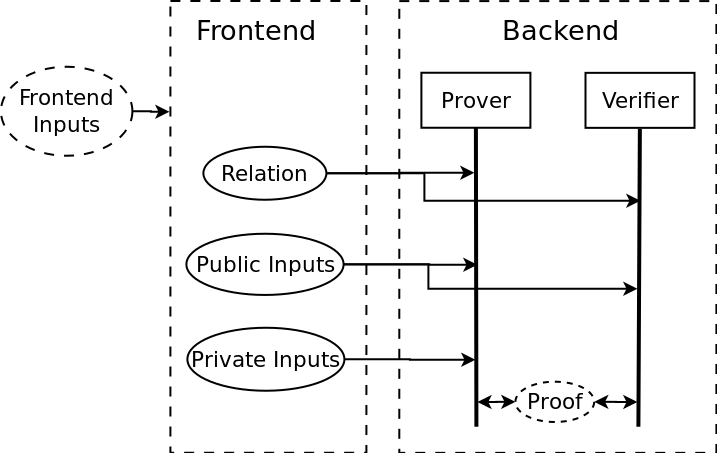
\includegraphics[width=0.75\textwidth,center]{ir-dataflow-simple.png} \\

\subsection{Genesis}

In the course of the SIEVE Program, performers experimented with a variety of representations ranging from very high level through very low level.
The SIEVE Program has proved statements on every platform from mobile web to gigantic cloud instances, with runtime taking anywhere from milliseconds to days to prove.
Additionally, SIEVE backends have preferred a wide variety of intermediate representations -- including R1CS, C++ compilation, and other custom solutions.
The greatest challenge in developing the IR has been making it flexible enough to accomodate so many requirements.

The program's first attempt at a flexible IR, the SIEVE IR v1.0, was to essentially overlay high-level features upon a flat circuit with numbered wires.
This was a failure for backends wanting just flat circuits because they were forced to unroll high level features.
It was also a failure for the higher level backends because the numbered wires were insufficient to convey high level meaning and long stretches of flat circuitry would cause slowdowns for them.

\subsection{Flexibility and Scalability}

To resolve this issue, the latest SIEVE IR revision has two layers.
The lower layer, called the Circuit-IR, defines a flat circuit, augmented with flat functions.
While it is not completely flat, it does strike a balance between statement size and interpreter complexity -- important because many SIEVE backends bottlenecked on disk IO while reading completely flat circuits.

A great strength of the Circuit-IR is circuit streaming.
Gates are processed one after the other, and their outputs (wires) are stored until needed for further computation.
Ordinarily, this would cause memory usage to increase until either the circuit ends or the available memory is exhausted.
The Circuit-IR implements memory management operations and restrictions which enables a circuit to declare what wires it will produce and when it is finished with them, so that its memory may be recycled.

The higher layer, called Translation-IR, is a fairly high level language in terms of control flow.
For maximal compatibility, SIEVE Performers are also developing a translation into the Circuit-IR, hence the name Translation-IR.
But the Translation-IR need not be translated just to the Circuit-IR, one of its goals is that it be translatable to non-SIEVE IRs such as the aforementioned R1CS, C++ compilation, or other custom solutions.
At the time of writing, the Circuit-IR recently survived the program's Phase II Testing Event, while the Translation-IR is currently in development.

\subsection{Multi Field Circuits}
To most practitioners of ZK, a single prime field is chosen at the beginning of a proof and used throughout.
However, for some applications it is desirable to use multiple primes for different elements within a single larger proof.
For example a large and expensive prime may be needed to verify public-key signatures, while a medium sized prime is necessary for large scale business logic.

To accommodate these applications, the IR must allow for multiple fields within a single relation.
To the frontend each field must describe the type of a wire, while to the backend these wires actually belong to multiple independent proofs.
An analogy to the real world might be a circuit card with transistor logic on one side and high voltage on the other.

Occasionally information from one field will be required in another.
The IR models this using a conversion gate with inputs in one field and outputs in another.
To continue the analogy, a relay would allow information to flow from transistor logic into high voltage, or in reverse, an analog-digital converter.
In ZK, methodologies must be developed and used to show equivalence of inputs and outputs across independent proofs or even across different proof systems.

\subsection{Resources of the SIEVE IR}
Each file or connection in the SIEVE IR is referred to as a resource, a stream of bytes to be consumed by the backend.
A relation is a resource, and so are the inputs to the relation.
There is also a special configuration resource which helps frontends and backends negotiate compatibility.

The SIEVE IR introduces two types of relation: the Circuit-IR and the Translation-IR.
\begin{itemize}
\item The Circuit-IR is defined by flat lists of gates and wires; functions may be defined and reused within the circuit.
\item The Translation-IR is a program which outputs a relation in the Circuit-IR format.
The backend is given some amount of control over how the Translation-IR is translated, and is free to reimplement common or standardized libraries, translate to an alternative IR, or even prove statements directly from the Translation-IR.
\end{itemize}

In recognition that many ZK backends can improve upon simple circuits' performance when particular functionality is desired, both layers of the IR define a \textbf{plugin} interface allowing calls from the IR into backend specific functionality.\\

To ease the frontends choice of configuration constants (such as prime fields and plugin parameters), a Circuit Configuration Communication occurs so that the backend may feed optimal constants to the frontend. \\

In total, the IR winds up with five resources: four in the frontend to backend direction, and a configuration which flows in the opposite direction.

\begin{itemize}
  \item Relation
  \begin{itemize}
     \item Translation-IR -- high level program which emits a flat circuit
     \item Circuit-IR -- flat circuit which is easy for backends to ingest
  \end{itemize}
  \item Public inputs -- a list of inputs known to both the Prover and Verifier
  \item Private inputs -- a list of inputs known only to the Prover
  \item Circuit Configuration Communication (CCC) - hints from the backend to the frontend describing features supported by the backend.
\end{itemize}

This illustration shows how the backends start by producing the CCC -- typically checked in with its source code -- enabling a frontend to choose types and plugins suitable to a backend.
Then the frontend can produce SIEVE IR enabling a web of available translations before the backend can finally prove the statement.

\noindent 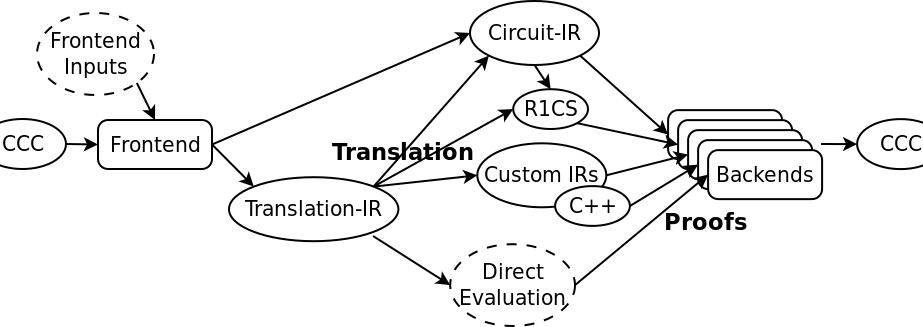
\includegraphics[width=0.95\textwidth,center]{ir-dataflow-translation.png} \\

%%%%
\section{Headers}
\label{sec:headers}

Please see the \textit{Headers} section of \textit{Introduction to the SIEVE Intermediate Representation}.

\section{Circuit-IR}
\label{sec:circuitir}

\subsection{Header}
\label{subsec:headers}

As stated in \Cref{sec:headers}, the Circuit-IR header starts with the version number and resource type.
\begin{lstlisting}[language=ir]
version 2.0.0;
circuit;
\end{lstlisting}
Next, all plugins (\Cref{sec:plugins}), types, and conversion gates that are used in the file are declared up front in the header, before
the \texttt{@begin} keyword.
The order of these declarations must be sorted.
Plugins must appear first, followed by types, and then conversion gates come last.

A type declaration specifies the types that are used in the rest of the file.
Types can specify either a \texttt{field}, \texttt{ext\_field}, or \texttt{ring}, as defined in \Cref{sec:types}.
Type declarations also implicitly specify a type-index, assigned incrementally as each type is specified. The maximum number of types that can be defined is \maxfieldcount.

It is a failure of resource validity to declare the same type more than once. This property allows backends to compare types by comparing indices, which is less computationally expensive
(in particular when dealing with large primes or structured types defined by plugins).

\begin{lstlisting}[language=ir]
// index 0: Boolean
@type field 2;
// index 1: 2^61 - 1
@type field 2305843009213693951;
// index 2: GF(2^63) with polynomial modulus x^63 + x + 1
@type ext_field 0 63 9223372036854775811;
// index 3: Ring over 2^32
@type ring 32;
\end{lstlisting}
%
This example declares two field types for the Boolean and $2^{61}-1$ prime fields, extension field type for $GF(2^{63})$, and a ring type for $2^{32}$, respectively indexed by 0, 1, 2, and 3.

All conversion gates used in the file must be declared in the header.
Each conversion gate declaration specifies which fields are converted between and how many of each field is input and output.
Note that the length of input and output ranges must be greater than 0.
Here are a few examples.
%
\begin{lstlisting}[language=ir]
// Convert Booleans to Mersenne61 and back
@convert(@out: 1:1, @in: 0:61);
@convert(@out: 0:61, @in: 1:1);
// Convert Mersenne61 to 25519 and back
@convert(@out: 1:5, @in: 2:1);
@convert(@out: 2:1, @in: 1:5);
\end{lstlisting}
Conversion gates are fully specified in \cref{subsec:conversiongates}.

\subsection{Types}\label{sec:types}

The Circuit-IR supports multiple types, as specified below.
\begin{itemize}
  \item \texttt{@type field <p>}: This type specifies a field modulo prime
        \texttt{p}.

        Examples:
        \begin{lstlisting}[language=ir]
// index 0: Boolean
@type field 2;
// index 1: 2^61 - 1
@type field 2305843009213693951;
        \end{lstlisting}

  \item \texttt{@type ext\_field <index> <degree> <modulus>}: This type
        specifies an extension field $GF(p^n)$, where \texttt{index} denotes the
        type index of the (non-extension) field $p$, \texttt{degree} denotes the
        degree $n$ of the extension field's polynomial modulus, and
        \texttt{modulus} is an integer constant which denotes the irreducible
        polynomial modulus of the extension field, as explained below. The value
        of \texttt{modulus} MUST be less than $p^n$, and the value of
        \texttt{index} MUST be associated with an already defined type.

        \medskip\noindent\textbf{Constant representation.} For extension fields,
        constants (including the \texttt{modulus} value above) are represented
        as base-10 integers, where the coefficients are the digits of the
        integer when interpreted in the base field $p$. The coefficient for the
        $X^k$ term is given by the $k$th digit of the constant written in base $p$,
        where the 0th digit is the least significant.

        As an example, for $GF(2^{63})$ the constant 9223372036854775811 denotes
        the polynomial $X^{63} + X + 1$.

        Examples:
        \begin{lstlisting}[language=ir]
// index 0: Boolean
@type field 2;
// index 1: GF(2^63) with polynomial modulus x^63 + x + 1
@type ext_field 0 63 9223372036854775811;
        \end{lstlisting}

  \item \texttt{@type ring <width>}: This type specifies a ring, $\mathbb{Z}_{2^n}$.
        Practically, these act like conventional unsigned base-2 integers.

        Examples:
        \begin{lstlisting}[language=ir]
// index 0: unsigned 32-bit integers
@type ring 32;
        \end{lstlisting}
\end{itemize}


\subsection{Public and Private Inputs}
Inputs to the circuit are provided through separate resources (See Section \ref{sec:streams}) and accessed as streams.
There are two streams per type, one for public inputs and one for private (prover only) inputs.
%
Stream access uses the following syntax for public inputs:
\begin{lstlisting}[language=ir]
$out_0 [... $out_n] <- @public([type_idx]);
\end{lstlisting}
And the following syntax for private inputs:
\begin{lstlisting}[language=ir]
$out_0 [... $out_n] <- @private([type_idx]);
\end{lstlisting}
Items are read from the stream corresponding to the type index and assigned to
the associated output wires. If the type index is not specified, it defaults to
zero.

\subsection{Memory Management}

Backends that consume SIEVE IR are highly optimized.
To minimize their overhead in managing memory, the IR exposes primitives to allocate and deallocate ranges of memory.
There are strict restrictions
on memory management: many operations require a range of input or output wires
that are not only consecutive but also are part of the same allocation.
This allows optimized backends to ensure that the input or output wires are
stored in contiguous memory.
Two wires may have consecutive wire-numbers, but be non-contiguous in memory,
depending on the backend's internal memory management strategy.

Each type is given its own numbering space, with wire-numbers in the range of $0 ... 2^{64}-1$.
Most directives will use a type-index parameter to select in which type, and in which numbering-space, they will act.
For example, \texttt{0: \$123} and \texttt{1: \$123} may both be defined, with each wire residing in different numbering space due to their different types.

To allocate a range of wires explicitly, the \texttt{@new([ type\_idx: ] \$first ... \$last);} directive may be used.
This creates a new allocation containing exactly the wire numbers \texttt{\$first ... \$last},
but does not assign values to those wires.
Reads from uninitialized wires is a failure of resource validity.
The new allocation must not overlap any previous allocation.
If the type index is not specified, it defaults to zero.

%
\begin{lstlisting}[language=ir]
@new(1: $100 ... $200);
\end{lstlisting}

Directives that assign to wires will implicitly allocate the output wires if needed.
For a directive that assigns to a range of output wires \texttt{type\_idx: \$first ... \$last},
if all wires in the range are unallocated, it first creates an allocation as by
the directive \texttt{@new(type\_idx: \$first ... \$last)} and then assigns to
the newly-allocated wires.
If, instead, any of those wires were previously allocated, then they all must
be part of a single allocation; if only some of the wires in the range were
allocated, or different wires are part of different allocations, this is a
failure of resource validity.
This applies even for single wires; a single output wire such as \texttt{type\_idx: \$wire}
is treated as a one-element range \texttt{type\_idx: \$wire ... \$wire}.
If a directive has multiple output wire ranges, each is handled independently,
even if the ranges use consecutive numbers.

\begin{lstlisting}[language=ir]
// Assume no wires are previously allocated.

// Implicitly allocates the range $100 ... $199
$100 ... $199 <- @call(foo1);

// Implicitly allocates the single wire $200
$200 <- @call(foo2);

@new($300 ... $399);
// All wires $300 ... $399 are already allocated, so this does
// not implicitly allocate.
$300 ... $399 <- @call(foo3);

@new($400 ... $449);
// Error: only some of the wires are allocated.
$400 ... $499 <- @call(foo4);

@new($500 ... $549);
@new($550 ... $599);
// Error: wires are not all part of a single allocation.
$500 ... $599 <- @call(foo5);

// This creates a separate allocation for each output range.
$600 ... $649, $650 ... $699 <- @call(foo6);
\end{lstlisting}
%stopzone

The \texttt{@delete} directive deallocates wires with the form \texttt{@delete([ type\_idx: ] \$first ... \$last );}.
All wires in the range \texttt{type\_idx: \$first ... \$last} must be assigned
and must not have been previously deleted.
The range may span multiple allocations, but it must cover each allocation in
full; deallocating only part of an allocation is a failure of resource
validity.
If the type index is not specified, it defaults to zero.

%
\begin{lstlisting}[language=ir]
// Set up some allocations
@new(1: $100 ... $199)
@new(1: $200 ... $299)
// Implicit allocations are treated the same as @new
$300 ... $399 <- @call(foo)

// Error: @delete includes wires that were never allocated
@delete(1: $300 ... $499)

// Error: @delete covers only part of the $300 ... $399 allocation
@delete(1: $300 ... $310)

// Delete the entire $100 ... $199 allocation
@delete(1: $100 ... $199)

// Delete the $200 ... $299 and $300 ... $399 allocations
@delete(1: $200 ... $399)
\end{lstlisting}

Once a wire has been deleted, its wire number may not be reused and it may not be deleted again.

\paragraph{IMPORTANT} Notice that the form of nearly all ranges in the IR is \texttt{first ... last} rather than \texttt{first ... length}.
Ranges are inclusive on both ends.


\subsection{Standard Gates}
\label{subsec:standardgates}
The form of most gates, unless otherwise specified, is:
\begin{lstlisting}[language=ir]
$out <- gate_name([ type_idx:] $left_in, $right_in);
\end{lstlisting}
For a circuit to be well-formed, the type index must refer to a valid declared type.
The type index is optional and defaults to type \texttt{0} when omitted.
Other gates have variations on this form, and are described as necessary.\\

\begin{itemize}
  \item \texttt{@add} field or ring addition
  \item \texttt{@mul} field or ring multiplication
  \item \texttt{@addc} field or ring addition by a constant
        \begin{lstlisting}[language=ir]
$out <- @addc([type_idx:] $left_in, <right_constant>);
        \end{lstlisting}

        \textbf{Note:} If \texttt{type\_idx} specifies an extension field, then
        \texttt{right\_constant} contains a decimal encoding of the extension
        field value, as is explained in \Cref{sec:types}.
  \item \texttt{@mulc} field or ring multiplication by a constant
        \begin{lstlisting}[language=ir]
$out <- @mulc([type_idx:] $left_in, <right_constant>);
            \end{lstlisting}

        \textbf{Note:} If \texttt{type\_idx} specifies an extension field, then
        \texttt{right\_constant} contains a decimal encoding of the extension
        field value, as is explained in \Cref{sec:types}.
    \item Copy the input wires to the output wires. The total number of input and output wires must be the same. Input and output ranges for copy gates must conform to the same memory contiguity constraints as input and output ranges for function calls as defined in \Cref{sec:funccall}.
        \begin{lstlisting}[language=ir]
$out_0 [... $out_n] <- [type_idx_0:]
                       $in_first_0 [... $in_last_0]
                       [, $in_first_m [ .. $in_last_m]];
        \end{lstlisting}
  \item Assign the input constant to the output wire
        \begin{lstlisting}[language=ir]
$out <- [type_idx:] <constant>;
        \end{lstlisting}

        \textbf{Note:} If \texttt{type\_idx} specifies an extension field, then
        \texttt{constant} contains a decimal encoding of the extension
        field value, as is explained in \Cref{sec:types}.
  \item \texttt{@assert\_zero} assert that a field element is zero
        \begin{lstlisting}[language=ir]
@assert_zero([type_idx:] $wire);
        \end{lstlisting}
\end{itemize}

For simplicity Boolean gates (in $GF(2)$) are replaced with mathematically equivalent arithmetic operations.
This table summarizes alternative gates. \\

\noindent\begin{tabular}{|c|c|}
  \hline
  \textbf{Boolean Gate} & \textbf{Arithmetic Replacement} \\
  \hline
  \verb|@and|           & \verb|@mul|                     \\
  \verb|@xor|           & \verb|@add|                     \\
  \verb|@not|           & \verb|@addc(x, <1>)|            \\
  \hline
\end{tabular} \\

For a circuit to be well formed, two rules must be obeyed when using and assigning wires.
First, \textbf{topological ordering} requires that when a wire is used as the input to a gate, it must have been previously defined by an earlier gate in the scope.
Second, \textbf{single static assignment (SSA)} requires that within a scope a particular wire is never redefined after its original assignment, even if it removed with the \texttt{@delete} directive.\\

\subsection{Conversion Gates}
\label{subsec:conversiongates}
Conversion gates enable conversion of wires from one type to another.
Conversion gates are only supported between two \texttt{field} types or between
an \texttt{ext\_field} type and its associated \texttt{field} type.

\subsubsection{Conversions Between Field Types}
Conceptually a list of wires in field A is converted to a list of wires in field B.
Within the circuit, a conversion gate has the form:
\begin{lstlisting}[language=ir]
out_type_idx: $out_first [... $out_last] <- @convert(
    in_type_idx: $in_first [... $in_last] [, @modulus|@no_modulus]);
\end{lstlisting}
The optional \texttt{@modulus} / \texttt{@no\_modulus} specifier specifies the semantics of the conversion; any other value denotes an error.
If not specified, we default to \texttt{@no\_modulus}.
%
The conversion's fields and number of wires must match a conversion specification from the front matter. If it is not the case, there is a resource invalidity.
Here is an example that uses conversion gates:
\begin{lstlisting}[language=ir]
version 2.0.0;
circuit;
// field 0: Boolean
@type field 2;
// field 1: 2^61 - 1
@type field 2305843009213693951;
// field 2: 2^255 - 19
@type field 57896044618658097711785492504343953926634992332820282019728792003956564819949;
// Declare used convert gates
@convert(@out: 1:1, @in: 0:61);
@convert(@out: 1:5, @in: 2:1);
@begin
    ...
    // convert Booleans to a single Mersenne61
    1: $0 <- @convert(0: $1 ... $61);
    // convert a single 25519 to 5 Mersenne61s
    1: $1 ... $5 <- @convert(2: $0);
    ...
@end
\end{lstlisting}
%
The input range \texttt{in\_type\_idx: \$in\_first ... \$in\_last} must be part
of a single allocation.
The output range \texttt{out\_type\_idx: \$out\_first ... \$out\_last} must
either be part of a single allocation or be unallocated; if it is unallocated,
the range will be implicitly allocated, as with \texttt{@new}.

\medbreak\noindent\textbf{Conversion Semantics.}\label{sec:conversion-semantics}
Here, we define in detail the specification of a \texttt{@convert} gate.
Inputs and outputs are expressed in big endian representation.
There are two possible semantics for conversions:
\begin{itemize}
  \item \texttt{@no\_modulus} (overflow semantics):
        To convert p wires $x_1 ... x_p$ in field A into q wires $y_1 ... y_q$ in field B, we first convert the p wires in field A into a natural number $N = \sum_{i=1}^p x_i \times A^{p-i}$.
        Then we try to represent $N$ using q wires in field B $y_1 ... y_q$ as $N = \sum_{i=1}^q y_i \times B^{q-i}$.
        If $N$ cannot be represented in this fashion, this constitutes a proof failure.

  \item \texttt{@modulus} (modulus semantics):
        To convert p wires $x_1 ... x_p$ in field A into q wires $y_1 ... y_q$ in field B, we first convert the p wires in field A into a natural number $N = \sum_{i=1}^p x_i \times A^{p-i} \mod B^q$.
        Then we represent $N$ into q wires in field B $y_1 ... y_q$: $N = \sum_{i=1}^q y_i \times B^{q-i}$.
\end{itemize}

\subsubsection{Conversions Between Extension Field and its Base Field}

For extension fields one can only convert between an extension field $GF(p^n)$ and its base field $p$.
\begin{lstlisting}[language=ir]
  out_type_idx: $out_first [... $out_last] <-
      @convert(in_type_idx: $in_first [... $in_last]);
\end{lstlisting}
Note that unlike for conversion gates for the field type, there is no optional
specifier in this case.

The conversion semantics are straightforward: when converting to the base field,
the extension field $GF(p^n)$ is decomposed into a sequence of $n$ wires of
field type $p$. When converting to the extension field, the $n$ wires of field
type $p$ are used to represent the polynomial coefficients in $GF(p^n)$. For
both conversion directions the base field wires use little endian ordering; that
is, \texttt{\$out\_first} represents the coefficient for $X^n$ and
\texttt{\$out\_last} represents the coefficient for $X^0$.

\begin{lstlisting}[language=ir]
version 2.0.0;
circuit;
// index 0: Boolean
@type field 2;
// index 1: GF(2^63)
@type ext_field 0 63 9223372036854775811;
// Declare used convert gates
@convert(@out: 0:63, @in: 1:1);
@convert(@out: 1:1, @in: 0:63);
@begin
  ...
  // convert Booleans to polynomial in GF(2^63)
  1: $0 <- @convert(0: $1 ... $63)
  // convert GF(2^63) to polynomial coefficients
  0: $1 ... $63 <- @convert(1: $0)
  ...
@end
\end{lstlisting}

\subsubsection{Conversion Between Rings and Fields}
Ring to ring, ring to field, and field to ring conversion use the same syntax as field to field conversions.
Each ring wire is to be treated as a vector of $n$-many $GF(2)$ values, in most significant bit first order, where $n$ is the bit-width specified in its type declaration.
Conversion can then proceed as a field to field conversion.

\subsection{Function Gates}

Function gates define a sub-circuit which may be reused multiple times.
The function's outputs and inputs are given as ranges mapped sequentially, and by type, into the function's scopes.
In the function's signature, each range is defined by a length and a type index.
When the function is invoked, each range is mapped into its scope incrementally from 0.

Function declaration and invocation have the following forms:
%
\begin{lstlisting}[language=ir]
@function(function_name,
    [@out: out_type_idx_0: out_field_count_0
	    [, out_type_idx_n: out_field_count_n],]
    [@in: in_type_idx_0: in_field_count_0
	    [, in_type_idx_n: in_field_count_n],]
    )
  /* gate list */
@end

[$out_first_0 [ ... $out_last_0 ]
  [, $out_first_n [ ... $out_last_n ] ] <- ]
  @call(function_name [, $in_first_0 [ ... $in_last_0 ]
      [, $in_first_n [ ... $in_last_n ] ] ]);
\end{lstlisting}
The length of input and output ranges must be greater than 0 (for all \texttt{i}, $\texttt{out\_field\_count\_i} > 0$ and $\texttt{in\_field\_count\_i} > 0$).

Note that function invocations do not specify the type index for inputs and outputs since they can be inferred from the function signature.

\subsubsection{Function Gate Example}
\label{sec:funccall}
\begin{lstlisting}[language=ir]
@function(dot_prod_10, @out: 1:1, @in: 1:10, 1:10)
  // omitted
@end

@new(1: $0 ... $9);
@new(1: $10 ... $22);
// assign $0 ... $19

$25 <- @call(dot_prod_10, $0 ... $9, $10 ... $19);
\end{lstlisting}
%stopzone

The \texttt{@call} directive must have one range of input wires for each input
range declared in the \texttt{@function} declaration.
Each range of input wires must be part of a single allocation.
Similarly, the \texttt{@call} must have one range of output wires for each
output range declared in the \texttt{@function}.
Each range of output wires must either be part of a single allocation or be
unallocated; if it is unallocated, the range will be implicitly allocated, as
with \texttt{new}.

\subsubsection{Function Declaration Ordering and Recursion}
Functions are declared at the top level of the circuit.
Function names come into scope after their declaration.
This prevents recursive functions and allows type checking while processing the file as a stream.
%
For example, the following invocation is valid.
\begin{lstlisting}[language=ir]
@function(a) /* ... */ @end

@function(b)
  @call(a);
@end

@call(b)
\end{lstlisting}
The next example is invalid since the function \texttt{a} has not been declared and is not yet in scope when \texttt{b} is defined.
\begin{lstlisting}[language=ir]
@function(b)
  @call(a);
@end

@function(a) /* ... */ @end

@call(b)
\end{lstlisting}

\subsection{Example}\label{sec:circuitir_example}
Here is a full example of a right-triangle using the Circuit-IR.
%
\begin{lstlisting}[language=ir]
version 2.0.0;
circuit;
@type field 7;
@type field 127;
@convert(1:1, 0:1);

@begin
  // mod 7 hypotenuse
  $0 <- @public(0);
  // mod 7 legs
  $1 <- @private(0);
  $2 <- @private(0);

  // mod 7 is too small to square them
  1:$0 <- @convert(0:$0);
  1:$1 <- @convert(0:$1);
  1:$2 <- @convert(0:$2);

  // square them
  $3 <- @mul(1: $0, $0);
  $4 <- @mul(1: $1, $1);
  $5 <- @mul(1: $2, $2);
  $6 <- @add(1: $4, $5);

  // invert the hypotenuse
  $7 <- @mulc(1: $3, <126>);

  // assert equal
  $8 <- @add(1: $6, $7);
  @assert_zero(1: $8);
@end
\end{lstlisting}

\subsection{Circuit Semantics and Validity}\label{circuit_ir_validity}
When working with the Circuit-IR there are three levels of semantics and validity to be considered.
Each level builds upon the prior level.

\begin{enumerate}
  \item \textbf{Syntactic Validity:} The IR resource is recognizable in the language defined by the IR's grammar (see appendix \ref{text_syntax} and \ref{binary_syntax}).
  \item \textbf{Resource Validity:} The IR resource obeys semantic rules which are falsifiable with just the single resource.
  \item \textbf{Evaluation Validity:} Three IR resources (relation, public inputs, and private inputs) obey semantic rules which are only falsifiable in tandem.
\end{enumerate}

While syntactic validity is important, it is easy to check using off the shelf parsing tools.
The focus of this subsection is on resource validity and evaluation validity.

Each resource is checked individually for \textbf{Circuit Well-formedness} or \textbf{Stream Well-formedness} (See Section \ref{sec:streams} for details).
Circuit Well-formedness focuses on ensuring that wires are connected correctly -- a ``broken'' wire would make the circuit poorly-formed -- and that all declared types are unique.

\begin{description}
  \item[Type Uniqueness] No type is declared more than once.
  \item[Topological Ordering] For a wire to be the input to a gate, it must have previously been assigned as an output wire within the same scope.
  \item[Static Single Assignment] Each wire which is allocated must be assigned exactly once within its scope.
  \item[Allocation of Range Arguments] When passing a range of wires (as either an input or an output), all wires in the range must belong to the same allocation, and the range's cardinality must match the called function or conversion gate's specification.
  \item[Deletion of Whole Allocations] When passing a range of wires to a \texttt{@delete} directive, all wires within the range must have previously been assigned and all allocates within the range must be whole allocations. E.g. a \texttt{@delete} directive may not split an allocation into smaller portions.
\end{description}

To meet \textbf{Evaluation Validity}, all three resources are evaluated together, and the following conditions must be met.

\begin{description}
  \item[Assertions] Each input to an \texttt{@assert\_zero} directive must carry the value $0$.
  \item[Stream Length Requirement] When the end of the circuit is reached each stream has exactly zero items remaining: it must not have run out of items before reaching the end, and there may not be any extra items.
\end{description}

%%%%

\section{Plugins}
\label{sec:plugins}

\subsection{Motivation}

% Why we need plugins
In the previous section, we describe the Circuit-IR which contains the core IR functionalities.
In this intermediate representation, we would like to add some (complex) features (e.g. RAM operations).
Unfortunately, each update in the basic syntax forces frontends and backends to update their IR generator and parser.
We would like to avoid this burden while increasing expressibility of the language.
The goal of plugins is to allow IR extensions without changing the core IR.

\subsection{Plugin Syntax}
Plugins allow a circuit to refer to specific functionalities.
Those functionalities are defined in a document.
Only backends that have an implementation of a plugin can evaluate statements containing that plugin.

In the circuit's syntax, plugins are similar to functions except the function body is replaced by the plugin.
The declaration of a plugin function starts with the signature of a function followed by the use of a \texttt{@plugin} directive with plugin parameters that includes the plugin name, the operation name, and its generic parameters.
Invocation will remain the same as for functions.
A function bound to a plugin must be declared before its invocation.

The names of plugins used % (e.g. vector, matrix, ram\_write)
must be specified in the header. % before the `@begin` keyword.
This ensures that backends can easily check which plugins are used and reject the circuit if needed, prior to starting circuit evaluation.

 % Examples
 Here is an example use of the \texttt{vectors\_v1} plugin that provides a \texttt{mul} operation over ranges of wires.
\begin{lstlisting}[language=ir]
...
@plugin vectors_v1;
...
@begin
  ...
  // declare the function signature with a plugin body
  @function(vec_mul_4, @out: 0:4, @in: 0:4, 0:4)
      @plugin(vectors_v1, mul);
  ...
  // call the vec_mul_4 plugin function
  $8 ... $11 <- @call(vec_mul_4, $0 ... $3, $4 ... $7);
  ...
@end
\end{lstlisting}

Plugin operations are defined elsewhere, so the \texttt{@plugin} binding takes a list of plugin defined arguments after the required plugin and operation names.
Function signatures and their calls (\texttt{@call}) remain well-specified in the IR.
Each instantiation of a plugin operation % that's used in the circuit 
requires a separate function declaration and \texttt{@plugin} binding.
Plugin binding arguments consist of a comma separated sequence
of identifiers and numeric literals.
In practice, this enables plugins to specify parameters like fields, lengths, and other functionality.
Providing other functions' names as generic arguments can enable higher order operations like maps and folds. 
%
\begin{lstlisting}[language=ir]
/* ... */
@plugin vectors_v1;
@plugin iter_v0;
/* ... */
@begin
  /* ... */
  // Multiple instantiations of the same plugin (vector, mul)
  @function(vec_mul_4, @out: 0:4, @in: 0:4, 0:4)
      @plugin(vectors_v1, mul);
  @function(vec_mul_2, @out: 0:2, @in: 0:2, 0:2)
      @plugin(vectors_v1, mul);

  // Numeric parameter used as a circuit constant by the plugin
  @function(vec_double_4, @out: 0:4, @in: 0:4)
      @plugin(vectors_v1, mulc, 2);

  // Higher order map operation.
  @function(plus1_0, @out: 0:1, @in: 0:1) /* ... */ @end
  // An identifier parameter for the sub-function name,
  // A numeric parameter describing function arguments by their order
  // A numeric parameter for the iteration count
  @function(vec_plus1_4, @out: 0:4, @in: 0:4)
      @plugin(iter_v0, map, plus1_0, 0, 4);
  /* ... */
@end
\end{lstlisting}

Each plugin operation has a signature, which is defined as part of the standard for the plugin.
If the backend sees a \texttt{@plugin} for a known plugin, and the function signature doesn't match the expected signature of the operation it is being bound to, then the circuit is invalid. % the TA2 should reject the circuit with an error.
Further, the plugin's name must have been declared in the circuit header.
Either of these errors would make the circuit \textbf{poorly formed}.

Plugin operations may consume some public and private inputs. % instances and witnesses.
If a plugin operation consumes input from the standard public or private streams, its plugin binding
must contain the count of the number of consumed public or private inputs % instances and witnesses 
per field.
However, a plugin may be sophisticated enough to produce its own public or private inputs and consume them immediately, in which case input usage need not be declared.
%
Here is an example use of an \texttt{assert\_equal} plugin that checks that the five inputs are equal to the five next private inputs.
\begin{lstlisting}[language=ir]
/* ... */
@plugin assert_equal;
/* ... */
@begin
  /* ... */
  // declare the function signature with a plugin body
  @function(equal_to_private, @in: 0:5)
    @plugin(assert_equal, private, 0, 5, @private: 0:5);
  /* ... */
  // call the equal_to_private plugin
  @call(equal_to_private, $4 ... $8);
  /* ... */
@end
\end{lstlisting}

\subsection{Plugin Types}
%
For some plugins, it is useful to declare additional types that are distinct from ordinary field types.
Plugins can define new types by using the 
\texttt{@type @plugin(plugin\_id, type\_id, ...)} directive in the circuit header, which again takes a list of plugin-specified parameters. 
The first two parameters name the plugin, and a particular type within the plugin.
Subsequent parameters may be identifiers or numbers, and their semantics are defined by the plugin.
Types declared by a plugin can be manipulated via its plugin functions, or the plugin may overload built-in gates for its types.
Here is an example demonstrating how the \texttt{ram\_arith\_v1} plugin uses a plugin type to implement a buffer.

\begin{lstlisting}[language=ir]
version 2.0.0;
circuit;
@plugin ram_arith_v1;
// Wire type 0 is the field mod 127
@type field 127;
// Wire type 1 is the ram plugin type, with indexes and
// elements both drawn from field 0.
@type @plugin(ram\_arith\_v1, state, 0);

@begin
  // Declare RAM operations as abstract functions.
  // ram.init creates a buffer of fixed size and
  // initializes each element to the same input value.
  @function(ram_init, @out: 1:1, @in: 0:1) 
    @plugin(ram, init, 10);

  // ram.read takes an RAM buffer and an address
  // and returns the value at that address.
  @function(ram_read, @out: 0:1, @in: 1:1, 0:1)
    @plugin(ram_arith_v1, read);

  // ram_write takes a RAM buffer, an address, and
  // a new value and writes the value to the address.
  @function(ram_write, @in: 1:1, 0:1, 0:1)
    @plugin(ram, write);

  @function(assert_eq, @in: 0:1, 0:1)
    $2 <- @addc($0, <126>); // p-1
    $3 <- @add($1, $2);
    @assert_zero($3);
  @end

  // Initialize all elements to 0 (type 0) in a newly
  // allocated RAM buffer (type 1)
  $0 <- 0: <0>;
  $0 <- @call(ram_init, $0);

  // Write something to the address
  $1 <- @private_in(); // address
  $2 <- @private_in(); // value

  //             1:$0 RAM Buffer
  //                 0:$1 address wire
  //                     0:$2 value wire
  @call(ram_write, $0, $1, $2);

  // Read from the same address and check correctness.
  $3 <- @call(ram_read, $0, $1);
  @call(assert_eq, $2, $3);
@end
\end{lstlisting}


%%%%

\section{Input Streams}\label{sec:streams}
Public and private inputs are provided as separate resources. 
We have one input file per type and per visibility level (\texttt{public\_input} or \texttt{private\_input}).
These input files start with the same headers as described in \cref{sec:headers}: the version, the resource type (\texttt{public\_input} or \texttt{private\_input}), and one type.
Then, a sequence of numeric literals representing type elements is provided between \texttt{@begin} and \texttt{@end} tags.
These sequences act as a stream, and certain directives in the circuit % relation
consume a value from one of these streams.
If values in either stream are exhausted, this is a failure of evaluation validity.
If values remain in a stream after processing, then this is also an evaluation invalidity.
Here is an example for public and private inputs. 

\begin{lstlisting}[language=ir]
version 2.0.0;
public_input;
@type field 7;
@begin
  < 5 >;
@end
\end{lstlisting}
%
\begin{lstlisting}[language=ir]
version 2.0.0;
public_input;
@type field 19;
@begin
  < 2 >;
  < 15 >;
@end
\end{lstlisting}
%
\begin{lstlisting}[language=ir]
version 2.0.0;
private_input;
@type field 7;
@begin
  < 3 >;
  < 4 >;
@end
\end{lstlisting}

%%%%

\section{Circuit Configuration Communication (CCC)}

\subsection{Motivation}

To ease interoperation each backend should provide a configuration file declaring available types and plugins that the frontend may use.
This \textit{Circuit Configuration Communication}, or \textit{CCC} for short, is a static configuration file provided with the installation of a backend, and the frontend can configure from it while generating a statement.
The CCC starts with supported plugins, then types, conversions, and it may end with plugin constraints.
A compatible frontend will only use
\begin{itemize}
    \item the types supported by the targeted backend according to the CCC file,
    \item the standard gates (\Cref{subsec:standardgates}),
    \item the conversion gates supported by the targeted backend according to the CCC file, and
    \item the plugins supported by the targeted backend according to the CCC file.
\end{itemize}

All SIEVE IR compatible backends must provide a CCC, and all SIEVE IR compatible frontends must ingest a backend's CCC to generate a statement for the backend.
In the case that a backend cannot provide a feature (such as a type or a plugin) which the frontend would require, the frontend will be unable to generate a statement, and the pair of frontend and backend would be mutually incompatible.

\subsection{CCC content and syntax}

% 
A CCC file starts with the standard IR header (\Cref{sec:headers}), declaring its resource type as \texttt{configuration}.
It list the plugins, families of types, and conversion gates supported by the backend.

Each available plugin is specified by name using the same \texttt{@plugin plugin\_name;} syntax as the Circuit IR.
A plugins presence in the CCC indicates its availability, meaning that the frontend is allowed to use it, but it does not require the frontend to use it.
The frontend may use any subset of the backend's available plugins.
Similarly, a backend may indicate that no plugins are supported, by leaving the plugins list empty.

Here is an example plugin list indicating the availability of the \verb|mux_v0|, \verb|arith_ram_v0|, and \verb|arith_ram_v1| plugins.
Presumably, a frontend could then choose if to use the \verb|mux_v0| plugin, and if it needs RAM it could choose either version of the ram plugin.
The frontend could also use both versions of the RAM plugin, although that would be redundant and confusing.

\begin{lstlisting}[language=ir]
@plugin mux_v0;
@plugin ram_arith_v0;
@plugin ram_arith_v1;
\end{lstlisting}

\subsection{Type Families}\label{sec:families}

Types are grouped into ``type families'' in the CCC.
Each type family encompasses a set of types which are somehow related.
For example all fields which use Mersenne primes may be grouped into a ``Mersenne family''.

Each type family is specified first by what kind of type it is, then by predicates which constrain the set of possible types in the family.
A type family may be referenced later in the CCC by its index in the order in which they appear, same as how Circuit IR types are referenced.
There are four kinds of types, each having a different mathematical structure and accordingly different meanings for predicates.

\begin{itemize}
  \item A \texttt{field} type is defined by a single prime characteristic.
    Implicitly, the characteristic must be prime, and the predicates of a \texttt{field} family enforce further restrictions on it.
    A \texttt{field} family has the form \texttt{@type field(\textit{predicate} [, \textit{predicates...}]);}.
    An empty list of predicates (e.g. empty parenthesis) indicates that any prime is supported (including, for example, 7).
  \item An \texttt{ext\_field} type is defined by a base field, a polynomial order, and a numeric encoding of polynomial coefficients (see \Cref{sec:types}).
    There are three groups of predicates to an \texttt{ext\_field} family.
    The first group is a list of previously declared base \texttt{field} families, referenced by index.
    The base type of a member of this \texttt{ext\_field} family must be a member of one of the allowed base \texttt{field} families, but need not be a member of all (in fact, two base \texttt{field} families may be distinct of each other).
    The second group is predicates upon the order of the extension field.
    The order must be greater than one, and predicates may define additional restrictions.
    A third group defines predicates upon the numerically encoded polynomial coefficients.
    The polynomial must be irreducible, and predicates may define additional restrictions.
    An \texttt{ext\_field} family has the form \texttt{@type ext\_field (\textit{base\_idx} [, \textit{base\_idxs...}]) (\textit{predicate} [, \textit{predicates...}]) (\textit{predicate} [, \textit{predicates...}]);}.
    The family must define at least one \texttt{\textit{base\_idx}}, but both the order predicates and polynomial predicates may be empty.
  \item A \texttt{ring} type uses a ring over a $2^n$ modulus, providing the familiar bit representation for n-bit integers.
    The predicates of a \texttt{ring} family enforce restrictions on $n$.
    A \texttt{ring} family has the form \texttt{@type ring(\textit{predicate} [, \textit{predicates...}]);}.
    An empty list of predicates (e.g. empty parenthesis) indicates that any $n$ is supported.
  \item A \texttt{plugin} type is defined using plugins. Plugin type families use plugin constraints (see below) instead of predicates.
    A \texttt{plugin} family has the form \texttt{@type @plugin \textit{plugin\_name};}.
\end{itemize}

\subsection{Predicates}\label{sec:predicates}

Predicates define constraints upon numeric parameters of a type.
The following predicates exist.

\begin{itemize}
  \item \texttt{less\_than( numeric )} constructs a predicate requiring the parameter to be less than the specified value.
  \item \texttt{greater\_than( numeric )} constructs a predicate requiring the parameter to be greater than the specified value.
  \item \texttt{equals( numeric )} constructs a predicate requiring the parameter to equal the specified value.
  \item \texttt{is\_mersenne} is a predicate requiring that the parameter be a Mersenne prime.
  \item \texttt{is\_proth} is a predicate requiring that the parameter be a Proth prime.
  \item \texttt{is\_power\_of\_2} is a predicate requiring that the parameter be a power of two.
\end{itemize}

When a type uses multiple predicates, each predicate is ANDed with the others.
To produce an OR relation between predicates, simply create multiple type families.

\subsection{Conversion Declarations}\label{sec:ccc_conv_decl}

Conversion gate declarations specify which type families the backend supports conversions between.
Conversion gates are declared with \texttt{@convert(@out: family\_index\_out, @in: family\_index\_in);}, where the type families converted to and from are specified by their indices.
It is currently not possible to configure constraints on the number of input or output wires in a conversion.
% 

\subsection{Plugin Constraints}\label{sec:plugin_constraints}

Certain plugins may define additional constraints, such as constraints on
vector widths or RAM address and value types.
For each such plugin that the backend supports, the CCC should contain a
\emph{constraint block} delimited by \texttt{@plugin\_constraint(ram) ... @end}, containing
\texttt{@constraint(...)} lines specific to that plugin.
The arguments to each \texttt{@constraint} line consist of comma-separated identifiers and
integers, similar to the arguments of a function's \texttt{@plugin} binding
declaration.
Predicates may also be used within a \texttt{@constraint}, however their associativity and combinations with arbitrary identifiers or integers is plugin defined.
Each plugin that uses constraints will specify the structure and semantics of
\texttt{@constraint} lines allowed within the plugin's constraint block.

\subsection{Example}\label{sec:ccc_example}

\begin{lstlisting}[language=ir]
version 2.0.0;
configuration;

// The following plugins may be used
@plugin mux_v0;
@plugin ram_arith_v0;
@plugin ram_arith_v1;

// 0: The field of exactly 2
@type field(equals(2));

// 1: Any prime greater than 1 million
@type field(greater_than(1000000));

// 2: Any mersenne prime which is greater than 100 and less than 1000.
// To avoid confusion, for a Mersenne Prime p such that p = 2**m - 1,
// 100 < p < 1000, rather than m.
@type field(is_mersenne, greater_than(100), less_than(1000));

// 3: An extension field over GF(2**4)
@type ext_field (0) (equals(4)) ();

// 4: a 16, 32, or 64-bit unsigned integer
@type ring(is_power_of_2, less_than(65), greater_than(15));

// 5, 6: RAM Types for either the v0 or v1 RAM plugin
@type @plugin ram_arith_v0;
@type @plugin ram_arith_v1;

// Conversion from large fields (type 1) to Booleans (type 0)
@convert(@out: 0, @in: 1);

// Conversion from large primes (type 1) to Mersennes (type 2)
@convert(@out: 2, @in: 1);

// Conversions from the extension field (type 3) to Booleans (type 0)
// Note, that the IR only defines conversions involving extension
// fields to or from their base fields.
@convert(@out: 0, @in: 3);

// Bidirectional conversions of fields (type 1) and rings (type 4)
@convert(@out: 4, @in: 1);
@convert(@out: 1, @in: 4);

// Note that different versions of the same plugin are
// unlikely to be compatible
// INVALID: @convert(@out: 5, @in: 6);

// Note that although constraints are shown for the vectors_v1
// plugin, they are shown for demonstration purpose and are not
// standardized. Frontends are unlikely to recognize these
// constraints.

@plugin_constraints(vectors_v1)
  // Element type must match either of the first two @field lines.
  // The plugin spec defines the meaning of repeated element_type
  // constraints; in this case, we assume repeated lines are
  // allowed and that the constraint is satisfied if at least one
  // line is satisfied.
  @constraint(element_type, 0);
  @constraint(element_type, 1);

  // Vector width must be a power of two between 2 and 16.  The
  // meaning of these constraints is defined by the plugin spec.
  @constraint(vector_width, is_power_of_2, 2, 16);
@end
\end{lstlisting}


%%%%

\begin{appendices}

\section{Textual Syntax}\label{text_syntax}
This appendix uses a right-recursive BNF grammar to define the exact syntax of the text format.\\

\newcommand{\nterm}[1]{$\langle$#1$\rangle$}
\newcommand{\term}[1]{`#1'}

\subsection{Special Tokens} \label{appendix_special_tokens}
The following special tokens are defined by regular expressions.

\begin{alltt}
\nterm{number} => 0 ;
\nterm{number} => [1-9][0-9]* ;
\nterm{number} => 0x[0-9a-fA-F]+ ;
\nterm{number} => 0X[0-9a-fA-F]+ ;
\nterm{number} => 0o[0-7]+ ;
\nterm{number} => 0O[0-7]+ ;
\nterm{number} => 0b[0-1]+ ;
\nterm{number} => 0B[0-1]+ ;

// interpret `$' as a literal dollar sign (U+0024)
\nterm{wire-number} => $[1-9][0-9]* ;
\nterm{wire-number} => $0x[0-9a-fA-F]+ ;
\nterm{wire-number} => $0X[0-9a-fA-F]+ ;
\nterm{wire-number} => $0o[0-7]+ ;
\nterm{wire-number} => $0O[0-7]+ ;
\nterm{wire-number} => $0b[0-1]+ ;
\nterm{wire-number} => $0B[0-1]+ ;

// interpret `.' as a literal point or dot (U+002E)
\nterm{identifier} => [a-zA-Z_][a-zA-Z0-9_]*((.|::)[a-zA-Z_][a-zA-Z0-9_]*)* ;
\end{alltt}

Whitespace is defined with the following regular expression. Do note that in certain cases, non-empty whitespace may be necessary to break larger tokens.\\

\begin{alltt}
// * is repetition. {\textbackslash}* is a star character.
// {\textbackslash}n, {\textbackslash}r, {\textbackslash}t are newline, carriage return, and tab.
\nterm{whitespace} => ( |{\textbackslash}n|{\textbackslash}r|{\textbackslash}t|//[^{\textbackslash}n]*{\textbackslash}n|/{\textbackslash}*([^{\textbackslash}*]|{\textbackslash}*[^/])*{\textbackslash}*/)* ;
\end{alltt}

\subsection{Header}
The following grammar is given for the IR Header.

\begin{alltt}
\nterm{header} => \nterm{version-spec} \nterm{resource-id} ;

\nterm{version-spec} => \term{version} \nterm{number} \term{.} \nterm{number} \term{.} \nterm{number} \term{;} ;

\nterm{resource-id} => \term{circuit} \term{;} ;
\nterm{resource-id} => \term{translation} \term{;} ;
\nterm{resource-id} => \term{public_input} \term{;} ;
\nterm{resource-id} => \term{private_input} \term{;} ;
\nterm{resource-id} => \term{configuration} \term{;} ;
\end{alltt}

\subsection{Circuit-IR}
The following grammar is given for the Circuit-IR (resource id \texttt{circuit}).

\begin{alltt}
\nterm{circuit} => \nterm{header} \nterm{circuit-header} \nterm{circuit-body} EOF ;

\nterm{circuit-header} => \nterm{type-list} ;
\nterm{circuit-header} => \nterm{type-list} \nterm{conversion-list} ;

\nterm{type-list} => \nterm{type} \nterm{type-list} ;
\nterm{type-list} => \nterm{type} ;
\nterm{type} => \term{@type} \term{field} \nterm{number} \term{;} ;
\nterm{type} => \term{@type} \term{ext_field} \nterm{number} \nterm{number} \nterm{number} \term{;} ;
\nterm{type} => \term{@type} \term{ring} \nterm{number} \term{;} ;

// note that in @out: t:n (and likewise @in: t:n), n > 0
\nterm{conversion-list} => \nterm{conversion} \nterm{conversion-list} ;
\nterm{conversion-list} => \nterm{conversion} ;
\nterm{conversion} => \term{@convert} \term{(}
    \term{@out} \term{:} \nterm{number} \term{:} \nterm{number} \term{,}
    \term{@in} \term{:} \nterm{number} \term{:} \nterm{number} \term{,}
    \term{)} \term{;} ;

\nterm{circuit-body} => \term{@begin} \nterm{top-scope} \term{@end} ;

\nterm{top-scope} => \nterm{top-scope-item} \nterm{top-scope} ;
\nterm{top-scope} => \nterm{top-scope-item} ;

\nterm{top-scope-item} => \nterm{function-declaration} ;
\nterm{top-scope-item} => \nterm{directive} ;

\nterm{function-declaration} => \term{@function} \term{(} \nterm{identifier} \term{,}
    \term{@out} \term{:} \nterm{parameter-list} \term{,}
    \term{@in} \term{:} \nterm{parameter-list} \term{)}
    \nterm{function-scope}
    \term{@end} ;

\nterm{function-declaration} => \term{@function} \term{(} \nterm{identifier} \term{,}
    \term{@in} \term{:} \nterm{parameter-list} \term{)}
    \nterm{function-scope}
    \term{@end} ;

\nterm{function-declaration} => \term{@function} \term{(} \nterm{identifier} \term{,}
    \term{@out} \term{:} \nterm{parameter-list} \term{)}
    \nterm{function-scope}
    \term{@end} ;

\nterm{function-declaration} => \term{@function} \term{(} \nterm{identifier} \term{)}
    \nterm{function-scope}
    \term{@end} ;

// note that in parameter t:n, n > 0
\nterm{parameter-list} => \nterm{parameter} \term{,} \nterm{parameter-list} ;
\nterm{parameter-list} => \nterm{parameter} ;
\nterm{parameter} => \nterm{number} \term{:} \nterm{number} ;

\nterm{function-scope} => \nterm{function-scope-item} \nterm{function-scope} ;
\nterm{function-scope} => \nterm{function-scope-item} ;
\nterm{function-scope-item} => \nterm{directive} ;

\nterm{directive} => \nterm{new-directive} ;
\nterm{directive} => \nterm{delete-directive}
\nterm{directive} => \nterm{binary-gate} ;
\nterm{directive} => \nterm{binary-const-gate} ;
\nterm{directive} => \nterm{copy-directive} ;
\nterm{directive} => \nterm{assign-directive} ;
\nterm{directive} => \nterm{input-gate} ;
\nterm{directive} => \nterm{assert-zero-directive} ;
\nterm{directive} => \nterm{convert-gate} ;
\nterm{directive} => \nterm{call-directive} ;

\nterm{new-directive} => \term{@new} \term{(}
    \nterm{number} \term{:} \nterm{wire-number} \term{...} \nterm{wire-number} \term{)} \term{;} ;
\nterm{new-directive} => \term{@new} \term{(}
    \nterm{wire-number} \term{...} \nterm{wire-number} \term{)} \term{;} ;

\nterm{delete-directive} => \term{@delete} \term{(}
    \nterm{number} \term{:} \nterm{wire-number} \term{...} \nterm{wire-number} \term{)} \term{;} ;
\nterm{delete-directive} => \term{@delete} \term{(}
    \nterm{wire-number} \term{...} \nterm{wire-number} \term{)} \term{;} ;

\nterm{binary-gate} => \nterm{wire-number} \term{<-} \nterm{binary-gate-operation} \term{(}
    \nterm{number} \term{:} \nterm{wire-number} \term{,} \nterm{wire-number} \term{)} \term{;} ;
\nterm{binary-gate} => \nterm{wire-number} \term{<-} \nterm{binary-gate-operation} \term{(}
    \nterm{wire-number} \term{,} \nterm{wire-number} \term{)} \term{;} ;

\nterm{binary-gate-operation} => \term{@add} ;
\nterm{binary-gate-operation} => \term{@mul} ;

\nterm{binary-const-gate} => \nterm{wire-number} \term{<-} \nterm{binary-const-gate-operation} \term{(}
    \nterm{number} \term{:} \nterm{wire-number} \term{,} \term{<} \nterm{number} \term{>} \term{)} \term{;} ;
\nterm{binary-const-gate} => \nterm{wire-number} \term{<-} \nterm{binary-const-gate-operation} \term{(}
    \nterm{wire-number} \term{,} \term{<} \nterm{number} \term{>}  \term{)} \term{;} ;

\nterm{binary-const-gate-operation} => \term{@addc} ;
\nterm{binary-const-gate-operation} => \term{@mulc} ;

\nterm{copy-directive} => \nterm{wire-range} \term{<-} \nterm{number} \term{:} \nterm{wire-range-list} \term{;} ;
\nterm{copy-directive} => \nterm{wire-range} \term{<-} \nterm{wire-range-list} \term{;} ;
\nterm{assign-directive} => \nterm{wire-number} \term{<-} \nterm{number} \term{:} \term{<} \nterm{number} \term{>} \term{;} ;
\nterm{assign-directive} => \nterm{wire-number} \term{<-} \term{<} \nterm{number} \term{>} \term{;} ;

\nterm{input-gate} => \nterm{wire-range} \term{<-} \nterm{input-gate-operation} \term{(} \nterm{number} \term{)} \term{;} ;
\nterm{input-gate} => \nterm{wire-range} \term{<-} \nterm{input-gate-operation} \term{(} \term{)} \term{;} ;

\nterm{input-gate-operation} => \term{@public} ;
\nterm{input-gate-operation} => \term{@private} ;

\nterm{assert-zero-directive} => \term{@assert_zero} \term{(}
    \nterm{number} \term{:} \nterm{wire-number} \term{)} \term{;} ;
\nterm{assert-zero-directive} => \term{@assert_zero} \term{(} \nterm{wire-number} \term{)} \term{;} ;

\nterm{convert-gate} => \nterm{number} \term{:} \nterm{wire-range} \term{<-} \term{@convert} \term{(}
    \nterm{number} \term{:} \nterm{wire-range} \term{)} \term{;} ;

\nterm{wire-range} => \nterm{wire-number} ;
\nterm{wire-range} => \nterm{wire-number} \term{...} \nterm{wire-number} ;

\nterm{call-directive} => \nterm{wire-range-list} \term{<-} \term{@call} \term{(}
    \nterm{identifier} \nterm{wire-range-list} \term{)} \term{;} ;
\nterm{call-directive} => \term{@call} \term{(} \nterm{identifier} \nterm{wire-range-list} \term{)} \term{;} ;
\nterm{call-directive} => \nterm{wire-range-list} \term{<-} \term{@call} \term{(} \nterm{identifier} \term{)} \term{;} ;
\nterm{call-directive} => \term{@call} \term{(} \nterm{identifier} \term{)} \term{;} ;

\nterm{wire-range-list} => \nterm{wire-range} \term{,} \nterm{wire-range-list} ;
\nterm{wire-range-list} => \nterm{wire-range} ;
\end{alltt}

\subsection{Input Streams}
The following grammar is given for input streams (resources \texttt{private\_input} and \texttt{public\_input}).

\begin{alltt}
\nterm{stream} => \nterm{header} \nterm{stream-header} \nterm{stream-body} EOF ;

\nterm{stream-header} => \term{@type} \term{field} \nterm{number} \term{;} ;

\nterm{stream-body} => \term{@begin} \nterm{stream-list} \term{@end} ;
\nterm{stream-body} => \term{@begin} \term{@end} ;

\nterm{stream-list} => \nterm{stream-item} \nterm{stream-list} ;
\nterm{stream-list} => \nterm{stream-item} ;

\nterm{stream-item} => \term{<} \nterm{number} \term{>} \term{;} ;
\end{alltt}

\subsection{Circuit Plugins}
The following additions to the Circuit-IR grammar will enable plugins.

\begin{alltt}
\nterm{circuit-header} => \nterm{plugin-list} \nterm{type-list} ;
\nterm{circuit-header} => \nterm{plugin-list} \nterm{type-list} \nterm{conversion-list} ;

\nterm{plugin-list} => \nterm{plugin} \nterm{plugin-list} ;
\nterm{plugin-list} => \nterm{plugin} ;
\nterm{plugin} => \term{@plugin} \nterm{identifier} \term{;} ;

\nterm{type} => \term{@type} \nterm{plugin-binding} \term{;} ;

\nterm{function-declaration} => \term{@function} \term{(} \nterm{identifier} \term{,}
    \term{@out} \term{:} \nterm{parameter-list} \term{,}
    \term{@in} \term{:} \nterm{parameter-list} \term{)}
    \nterm{plugin-binding} \term{;} ;

\nterm{function-declaration} => \term{@function} \term{(} \nterm{identifier} \term{,}
    \term{@in} \term{:} \nterm{parameter-list} \term{)}
    \nterm{plugin-binding} \term{;} ;

\nterm{function-declaration} => \term{@function} \term{(} \nterm{identifier} \term{,}
    \term{@out} \term{:} \nterm{parameter-list} \term{)}
    \nterm{plugin-binding} \term{;} ;

\nterm{function-declaration} => \term{@function} \term{(} \nterm{identifier} \term{)}
    \nterm{plugin-binding} \term{;} ;

\nterm{plugin-binding} => \term{@plugin} \term{(} \nterm{identifier} \term{,} \nterm{identifier}
    \term{,} \nterm{plugin-arguments} \nterm{stream-count} \term{)} ;
\nterm{plugin-binding} => \term{@plugin} \term{(} \nterm{identifier} \term{,} \nterm{identifier}
    \nterm{stream-count} \term{)} ;

\nterm{plugin-arguments} => \nterm{plugin-argument} \nterm{plugin-arguments} ;
\nterm{plugin-arguments} => \nterm{plugin-argument} ;

\nterm{plugin-argument} => \nterm{number} ;
\nterm{plugin-argument} => \nterm{identifier} ;

\nterm{stream-count} => \term{,} \term{@private} \term{:} \nterm{stream-count-items} ;
\nterm{stream-count} => \term{,} \term{@public} \term{:} \nterm{stream-count-items} ;
\nterm{stream-count} => \term{,} \term{@private} \term{:} \nterm{stream-count-items} \term{,}
    \term{@public} \term{:} \nterm{stream-count-items} ;
\nterm{stream-count} => NULL ;

\nterm{stream-count-items} => \nterm{stream-count-item} \term{,} \nterm{stream-count-items} ;
\nterm{stream-count-items} => \nterm{stream-count-item} ;
\nterm{stream-count-item} => \nterm{number} \term{:} \nterm{number} ;
\end{alltt}

\section{Binary Syntax}\label{binary_syntax}

\subsection{FlatBuffer Schema}
The binary serialization of Circuit-IR will be described here using the \href{https://google.github.io/flatbuffers/}{open-source FlatBuffers cross-platform serialization library}, originally developed by Google.
FlatBuffers is a metaformat that specifies the superficial aspects of the syntax, such as representations of literals, structured data and arrays.
It moreover supports formal schemas that concretely define what elements (e.g., structures and arrays) can appear in the specific format.
FlatBuffers was chosen for the following reasons:
\begin{itemize}
    \item It offers an existing compact encoding of the format with efficient (de)serialization.
    \item It is supported by a wide-range of community-based tools and libraries for the most common languages (and is also easy to parse from scratch).
\end{itemize}

We will use the below FlatBuffers schema to represent \texttt{circuit}, \texttt{public\_input}, and \texttt{private\_input} resources. This schema is isomorphic to the Circuit-IR representation presented in Section~\ref{sec:circuitir}.

\lstinputlisting[language=flatbuffer]{sieve_ir.fbs}

As a structured format, the FlatBuffers schema provides a concrete, readable and typed syntax,
ensuring syntactic validity.
However, it does not provide resource or evaluation validity as it is not a language.
Refer to Section~\ref{circuit_ir_validity} to a description of syntactic, resource and evaluation validity.

\subsection{Multi Gigabyte Flatbuffer Limitations}
A limitation of the Flatbuffer technology is its 32-bit internal pointer representation, which prevents it from storing buffers larger than approximately 2GB.
The IR specifies the following workaround for this limitation.

\begin{itemize}
    \item The \texttt{Root} message may be repeated within a file or stream as many times as is necessary: each message holding a portion of the IR resource.
    \item Each message must be prefixed by its length in bytes, as a 4-byte unsigned little-endian number. (See \href{https://google.github.io/flatbuffers/class_flat_buffers_1_1_flat_buffer_builder.html#a425ab2bd13a0e4331a7190ec2d17c3b2}{FinishSizePrefix}).
    \item Each message's \texttt{version} attribute must be the same as the first message's \texttt{version}. All other attributes must be empty except for the resource's body.
\end{itemize}

Unfortunately, there is no way for a Flatbuffer to hold a single function which is larger than 2GB.

\end{appendices}



\end{document}
